\section*{Problem 1}
\subsection*{Part a}
The experimental data is normalized and fit to the the probability of being in $\ket{1}$ \ref{fig:rabi}
\eq{
\mathbb{P}_1 = ( \frac{\Omega^2}{\Omega^2 + (\omega - \omega_0)^2} )\sin^2 ( \sqrt{ \Omega^2 + (\omega - \omega_0)^2} t/2 )
}
The extracted Rabi angular frequency is $\Omega \approx 6.845 GHz$ and the angular resonant frequency is $\omega_0 \approx 57.759 GHz$.
\begin{figure}[h]
    \centering
    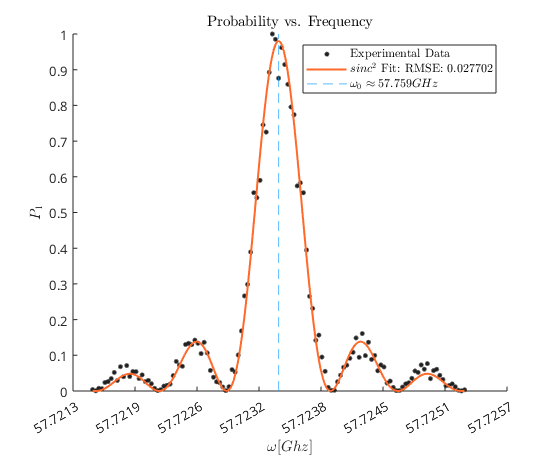
\includegraphics[width=1\linewidth]{Resources//245//Homework 4/245 Homework 4 Problem 1.png}
    \caption{Experimental data and curve fit for probability of measuring $\ket{1}$}
    \label{fig:rabi}
\end{figure}

\subsection*{Part b}
The uncertainty is, as RMSE, $0.027702$.

\section*{Problem 2}
\subsection*{Part a}
From Newton's law
\eq{
m ddt2x &= -kx\\
 ddt2x &= - k/m x\\
 ddt2x &= - \omega^2 x
}
Where $\omega = \sqrt{\frac{k}{m}}$.

\subsection*{Part b}
This is just a second order homogeneous ODE, the characteristic equation is
\eq{
r = \pm i \omega
}
So the general solution is
\eq{
x(t) &= C_1 e^{i \omega t} + C_2 e^{-i\omega t}\\
\dot{x}(t) &= i \omega C_1 e^{i\omega t} -i\omega C_2 e^{-i\omega t}
}
Plugging in the initial conditions
\eq{
x(0) &= C_1 + C_2\\
\dot{x}(0) &= i\omega C_1 - i\omega C_2\\
\implies C_1 &= 1/2 ( x(0) -i \omega \dot{x}(0) )\\
\implies C_2 &= 1/2 ( x(0) + i\omega \dot{x}(0) )
}
If we let
\eq{
A &= \sqrt{x^2(0) + (\omega \dot{x}(0))^2}\\
\phi &= \arctan ( \frac{\omega \dot{x}(0)}{x(0)})
}
Then the solution can be written as
\eq{
x(t) &= A/2 ( e^{i(\omega t+\phi)} + e^{-i(\omega t + \phi)} )\\
 &= A\cos( \omega t + \phi)
}

\subsection*{Part c}
The kinetic energy is
\eq{
KE(t) &= 1/2 m\dot{x}^2\\
 &= 1/2 mA^2\omega^2 \sin^2(\omega t + \phi)\\
 &= 1/2 k A^2 \sin^2(\omega t + \phi)
}

\subsection*{Part d}
The potential energy is
\eq{
PE(t) &= 1/2 k x^2\\
 &= 1/2 k A^2 \cos^2 (\omega t + \phi)
}

\subsection*{Part e}
The total energy is
\eq{
E &= KE + PE\\ 
&= 1/2 kA^2\sin^2(\omega^2 t + \phi) + 1/2 k A^2 \cos^2(\omega t + \phi)\\
&= 1/2 kA^2
}

\newpage
\subsection*{Part f}
The plots for $\omega = 2\pi \times 1 Hz$ and $m = 2kg$ are below
\begin{figure}[h]
    \centering
    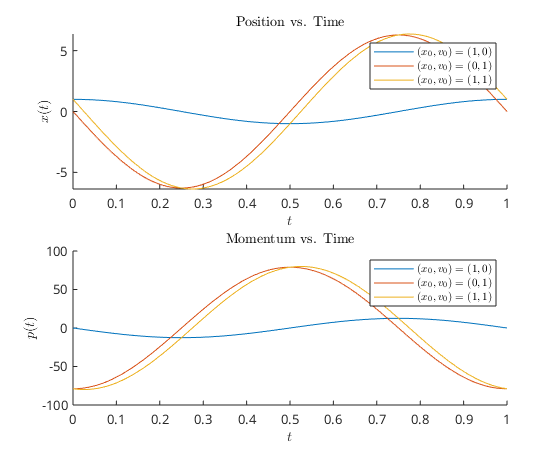
\includegraphics[width=1\linewidth]{Resources//245//Homework 4/245 Homework 4 Problem 2f.png}
    \caption{Enter Caption}
    \label{fig:enter-label}
\end{figure}

\newpage
\subsection*{Part g}
\begin{figure}[h]
    \centering
    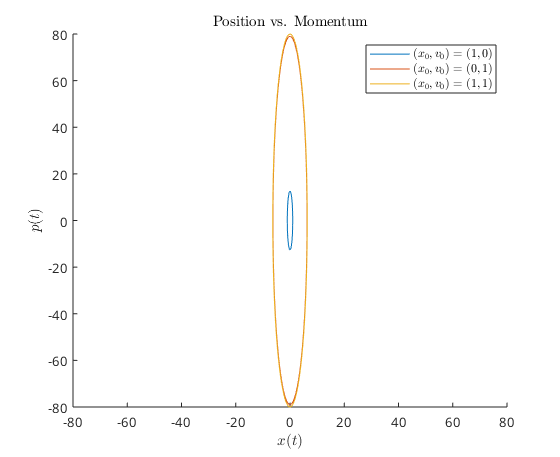
\includegraphics[width=1\linewidth]{Resources//245//Homework 4/245 Homework 4 Problem 2g.png}
    \caption{Enter Caption}
    \label{fig:enter-label}
\end{figure}

\newpage
\subsection*{Part h}
\begin{figure}[h]
    \centering
    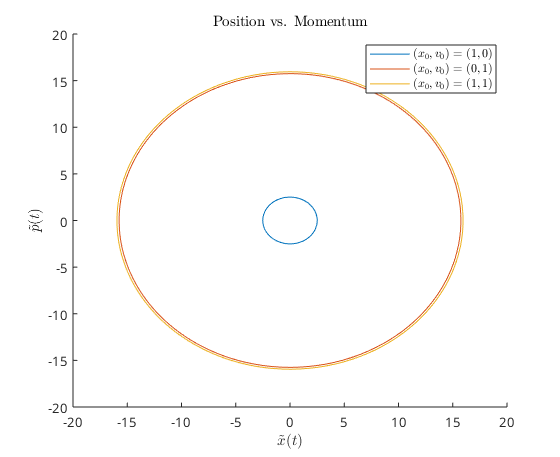
\includegraphics[width=1\linewidth]{Resources//245//Homework 4/245 Homework 4 Problem 2h.png}
    \caption{Enter Caption}
    \label{fig:enter-label}
\end{figure}

\subsection*{Part i}
In phasor notation we get
\eq{
z &= \sqrt{\frac{m\omega}{2}}x + \frac{i}{\sqrt{2m\omega}}p\\
&= \sqrt{\frac{m\omega}{2}x^2 + \frac{1}{2m\omega}p^2}e^{i \arctan( 1/2 \frac{x}{p})}\\
&= B e^{i\gamma}
}

\begin{figure}[h]
    \centering
    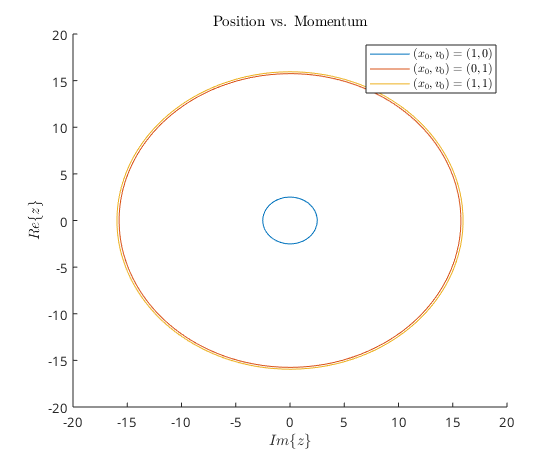
\includegraphics[width=1\linewidth]{Resources//245//Homework 4/245 Homework 4 Problem 2i.png}
    \caption{Enter Caption}
    \label{fig:enter-label}
\end{figure}

\section*{Problem 3}
\subsection*{Part a}
The expectation value of $x$ is
\eq{
\braket{x} &= \braket{n | \hat{x} | n}\\
&= \sqrt{\frac{\h}{2m\omega}}\braket{n | \hat{a} + \hat{a}^\dag | n}\\
&= 0
}
The expectation value of $p$ is
\eq{
\braket{p} &= \braket{n | \hat{x} | n}\\
&= -i\sqrt{\frac{\h m \omega}{2}}\braket{n | \hat{a} - \hat{a}^\dag | n}\\
&= 0
}
\subsection*{Part b}
The expectation value of $x^2$ is
\eq{
\braket{x^2} &= \frac{\h}{2m\omega}\braket{n | (\hat{a} + \hat{a}^\dag)^2 | n}\\
&= \frac{\h}{2m\omega} \braket{n | ( \hat{a}\hat{a}^\dag+\hat{a}^\dag\hat{a})|n}\\
&= \frac{\h}{2m\omega} (\braket{n | \hat{a}\hat{a}^\dag | n} + \braket{n|\hat{a}^\dag\hat{a}|n})\\
&= \frac{\h}{2m\omega} ( 2n +1 )\\
}

The expectation value of $p^2$ is
\eq{
\braket{p^2} &= -\frac{\h m\omega}{2}\braket{n | (\hat{a} - \hat{a}^\dag)^2 | n}\\
&= \frac{\h m\omega}{2} \braket{n | ( \hat{a}\hat{a}^\dag+\hat{a}^\dag\hat{a})|n}\\
&= \frac{\h m \omega}{2} (\braket{n | \hat{a}\hat{a}^\dag | n} + \braket{n|\hat{a}^\dag\hat{a}|n})\\
&= \frac{\h m \omega}{2} ( 2n +1 )\\
}

So the uncertainty is
\eq{
\sigma_x &= \sqrt{\frac{\h}{2m\omega} ( 2n +1 )}\\
\sigma_p &= \sqrt{\frac{\h m \omega}{2} ( 2n +1 )}
}

\subsection*{Part c}
\begin{figure}[h]
    \centering
    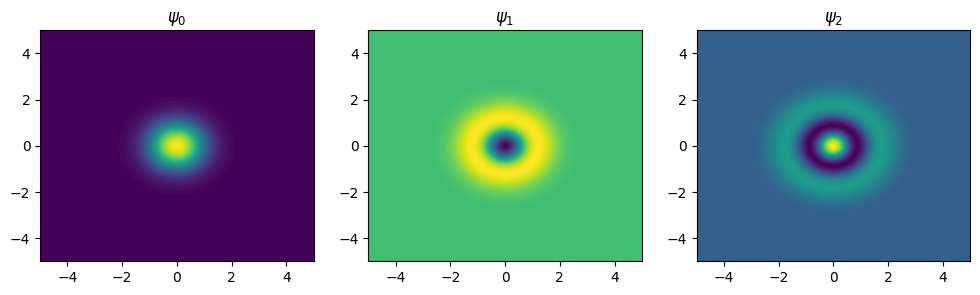
\includegraphics[width=1\linewidth]{Resources//245//Homework 4/245 Homework 4 Problem 3.png}
    \caption{Enter Caption}
    \label{fig:enter-label}
\end{figure}

\section*{Problem 5}
\subsection*{Part a}
From Newton's law we get
\eq{
m\Ddot{x} &= -kx + F_0 \cos (\omega t)
}
The easiest method for solving this ODE is Laplace Transforms
\eq{
s^2 X - x(0) -\dot{x}(0) +\omega^2 &= \frac{F_0}{m}\frac{s}{s^2+\omega^2}
}
\eq{
X &= \frac{F_0}{m} \frac{2\omega s}{(s^2+\omega^2)^2}\frac{1}{2\omega}+\frac{s}{s^2+\omega^2}x(0) + \frac{\omega}{s^2+\omega^2}\frac{\dot{x}(0)}{\omega}\\
x(t) &= \frac{F_0}{2m\omega}t\sin(\omega t) + x(0) \cos(\omega t) + \frac{\dot{x}(0)}{\omega}\sin(\omega t)\\
&= \sin(\omega t) (\frac{F_0}{2\omega}-m\omega x(0))+\cos(\omega t)(\frac{F_0}{2\omega}t + m\dot{x}(0))
}